\setchapterstyle{kao}
\setchapterpreamble[u]{\margintoc}
\chapter{Geometric Objects}
A geometric object is a physical thing who's identity is not dependant on human-imagined coordinates. Examples are velocity, EM fields, etc.
\section{Vectors}
In these notes, 4-vectors will be denoted by an arrow above a letter. It can be defined in three equivalent ways:
\begin{itemize}
    \item Coordinate independent object with magnitude and direction. An `arrow'. More generally, it is four independent numbers associated with each point in spacetime.
    \item A geometric object who's components transform like the components of an infinitesimal displacement. In this case,transform refers to transformation under a coordinate transformation.
    \item Tensor of type $\binom{1}{0}$. This is a linear function of a 1-form which return a real number.
\end{itemize}
The components of the vector $\Vec{A}$ are written as $A^\alpha$, i.e. $A^0, A^1,$ etc.
\subsection{Basis Vector}
Basis vectors are a special type of vector. For a 4-vector, there are 4 basis vectors, which are linearly independent, and ``point along'' \marginnote{Without a metric, angles cannot be measured. Therefore direction cannot be measured. In a metric-less setting, these basis vectors simply refer to  the coordinate axis.} the coordinate axis. They are written as
$$ \vec{e}_\alpha $$
these are vectors, not a component, which  will be explored more later. \par A full vector can therefore be written as
\begin{align*}
    \vec{A} &= A^\alpha \vec{e}_\alpha \\ &= A^0 \vec{e}_0 + \cdots + A^3 \vec{e}_3
\end{align*}
where the summation is implicit via the Einstein Summation Convention. \par Since basis vectors are vectors, they can be represented as
$$ \vec{e}_0 = \left(\vec{e}_\alpha \right)^\alpha $$
and due to linear independence between basis vectors, the identity between basis vectors \textbf{in the same basis} is
$$ \left( \vec{e}_\alpha \right)^\beta = \gvec{\delta}{\beta}{\alpha}  \quad \text{Kronecker Delta Function} $$

\subsection{Label Conventions}
There are housekeeping rules related to the indices. These are:
\begin{enumerate}
    \item Sides must balance, i.e. same number up and same number down either side of equality
    \item A pair of up and down indices are summations
    \item Never repeat indices more than once, i.e. $A^\alpha e_\alpha B^\alpha$ is not correct
\end{enumerate}

\subsection{Transformations of Vector Components}
Consider some primed coordinates $x^{\alpha'}$ and unprimed coordinates $x^\alpha$. The transformation from primed to unprimed coordinates is expressed by the transformation matrix, defined as 
$$ \gvec{\Lambda}{\alpha}{\beta'} \equiv \frac{\partial x^\alpha}{\partial x^{\beta'}} = 
\begin{bmatrix}
    \frac{\partial x^0}{\partial x^{0'}} & \dots & \frac{\partial x^0}{\partial x^{3'}} \\  \vdots & \ddots & \vdots \\ \frac{\partial x^3}{\partial x^{0'}} & \dots & \frac{\partial x^3}{\partial x^{3'}}
\end{bmatrix}
$$

\par Now consider some infinitesimal displacement $d\vec{x}$, the transformation of a component of a vector is defined as
\begin{definition}[Transformation of vector components]
    The transformation of the components of a vector from primed to unprimed coordinates, or vice versa, is given by
    \begin{align*}
        dx^\alpha & = \frac{\partial x^\alpha}{\partial x^{\alpha'}} \\ dx^{\alpha'} & = \frac{\partial x^{\alpha'}}{\partial x^\alpha} dx^\alpha
    \end{align*}
\end{definition}

\par Transformations are generally non-linear globally, but can be made linear locally.

\subsection{Position Vectors}
In general, position vectors do not transform similarly to perhaps a Lorentz boost. Position vectors generally don't exist, i.e. $\vec{A}$ is not a vector generally. \par With curved spacetime, there is more information needed to described the path of the position vector that the three numbers provided in a 4-vector. Hence, to be a vector, it must be a local quantity, and exist on the tangent space of the curved spacetime. \par Displacements (and all vectors) live locally in the tangent space of curved spacetime. See \vref{fig:tangent_space} for an illustration of this.
\begin{marginfigure}[-5cm]
    \centering
    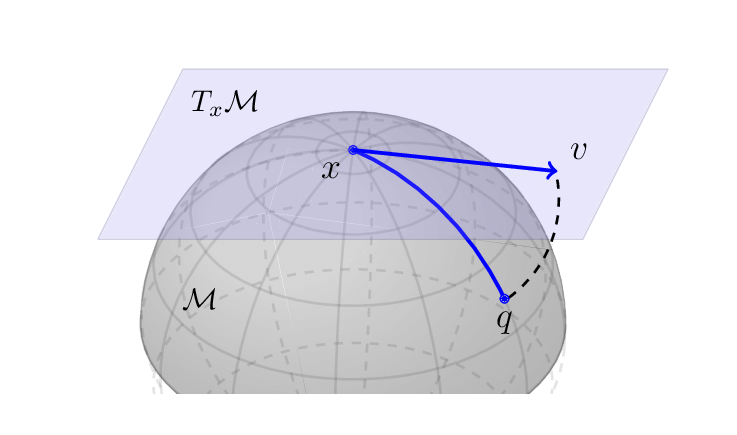
\includegraphics[width=\linewidth]{images/Figure-S3-Geometric-illustration-of-tangent-vector-tangent-space-curve-and.png}
    \caption{A hemispherical surface, $M$, with a tangent plane taken at point $z$. This tangent plane is in the tangent space of $M$.}
    \label{fig:tangent_space}
\end{marginfigure}

\subsection{Transformation of Basis Vectors}
Consider some arbitrary $\vec{A}$, with corresponding components and basis vectors
\begin{align*}
    \vec{A} & = A^\alpha \vec{e}_\alpha \\ & = A^{\alpha'} \vec{e}_{\alpha '} \\ & = \frac{\partial x^{\alpha'}}{\partial x^\alpha} A^\alpha \vec{e}_{\alpha'}
\end{align*}
Since $\vec{A}$ and $A^\alpha$ are equally arbitrary:
\begin{definition}[Transformation of Basis Vector]
    The transformation of a primed basis vector to unprimed basis vector is given by
    $$ \vec{e}_\alpha = \frac{\partial x^{\alpha'}}{\partial x^\alpha} \vec{e}_{\alpha'} $$
\end{definition}

\section{One-forms}
A 1-form, denoted by a letter with a tilde, e.g. $\widetilde{p}$, has three equivalent definitions, similar to vectors. These are:
\begin{itemize}
    \item A coordinate independent object with 4 linearly independent components, corresponding to the 4 coordinates in spacetime.
    \item A coordinate independent object, who's components transform like components of a gradient.
    \item A type $\binom{0}{1}$ tensor, which accepts vectors as arguments, and returns a real number.
\end{itemize}

Much like was mentioned earlier with vectors, a 1-form is a local object, since the contours that it represents must be straight. These contours must be evenly spaced and straight.
\subsection{One-form components}
A component of a 1-form is defined as 
$$ p_\alpha = \widetilde{p}(\vec{e}_\alpha) $$
Consider some arbitrary vector $\vec{A}$, and the relation between vectors and 1-forms can be shown as follows
\begin{align*}
    \widetilde{p}(\vec{A}) & = \widetilde{p}(A^\alpha \vec{e}_\alpha) \\ & = A^\alpha \widetilde{p}(\vec{e}_\alpha) && \text{(linearity)} \\ & = A^\alpha p_\alpha && \text{(definition)}
\end{align*}
There is a duality between vectors and 1-forms. They both exist in a tangent space for a point, and are dual to each other since a inner product may be taken between them. This inner product is the contraction
\begin{definition}[Inner Product]
    The contraction is an inner product, i.e.
    $$ \widetilde{p}(\vec{A}) = A^\alpha p_\alpha = \langle \widetilde{p}, \vec{A} \rangle $$
    Note that this is not the dot-product between vectors, since the dot-product requires a metric.
\end{definition}
$p_\alpha$ can be found then by creating a system of four simultaneous equations, and then solved to find each component.

\subsection{Transformation of 1-Forms Components}
Consider 1-form components of some primed index,
\begin{align*}
    p_{\alpha'} & = \widetilde{p}(\vec{e}_{\alpha'}) && \text{(definition)} \\
    & = \widetilde{p}\left(\frac{\partial x^\alpha}{\partial x^{\alpha'}} \vec{e}_\alpha \right) && \text{(change of vector basis)} \\ 
    & = \frac{\partial x^\alpha}{\partial x^{\alpha'}} \widetilde{p}  (\vec{e}_\alpha) && \text{(linearity)} \\ & = \frac{\partial x^\alpha}{\partial x^{\alpha'}} p_\alpha
\end{align*}
and thus it can be seen that 1-form components transform via the following identity
\begin{definition}[1-Form Component Transformation]
    The transformation of a 1-form components from a primed to unprimed space is given as
    $$ p_{\alpha} = \frac{\partial x^{\alpha'}}{\partial x^\alpha} p_{\alpha'} $$
\end{definition}

\subsection{Construction of $\widetilde{p}$ Components}
Similar to the vectors being constructed using basis vectors, the 1-forms are constructed using basis 1-forms.

\begin{definition}[Basis 1-Form]
    Basis 1-forms are written using the following notation
    $$ \gform{\omega}{\alpha} $$
    and are used to construct the 1-forms as follows
    $$ \widetilde{p} = p_\alpha  \gform{\omega}{\alpha} $$
\end{definition}

Similarly to basis vectors, the way to construct the basis 1-forms requires the formation of a family of linear equations, from which the values of the basis 1-forms can be found. 
\newpage
Now, consider an arbitrary vector $\vec{A}$ and 1-form $\widetilde{p}$:
\begin{align*}
        \widetilde{p}(\vec{A}) & = \widetilde{p}(A^\alpha \vec{e}_\alpha) && \text{(definition of vector} \\ 
        & = A^\alpha \widetilde{p}(\vec{e}_\alpha) &&\text{(linearity)} \\
        & = A^\alpha p_\beta \gform{\omega}{\beta} (\vec{e}_\alpha)
\end{align*}
Since $\vec{A}$ and $\widetilde{p}$ were taken to be arbitrary above,
$$ \gform{\omega}{\beta}(\vec{e}_\alpha) = \gvec{\delta}{\beta}{\alpha} $$
which forms a family of 16 linear equations which can be solved to find the 16 components of the 4 basis 1-forms.

\subsection{Transformation of Basis 1-Forms}
The basis 1-forms transform similarly to vector components
\begin{definition}[Transformation of Basis 1-Forms]
    $$ \gform{\omega}{\alpha'} = \frac{\partial x^{\alpha'}}{\partial x^\alpha} \gform{\omega}{\alpha} $$
\end{definition}

\subsection{1-Form Example}
The gradient 1-form is a common 1-form, somewhat analogous to the displacement vector. Consider some trajectory in spacetime, parameterised by an affine parameter, $\lambda$
$$ x^0(\lambda), \cdots, x^3(\lambda) $$
Similarly, consider an arbitrary scalar function, $\phi$, of the coordinates. The question is then of \textit{how does $\phi$ change along the trajectory?}
$$ \frac{d\phi}{d\lambda} = \frac{\partial \phi}{\partial x^\alpha} \frac{d x^\alpha}{d\lambda} $$
which is obvious via the chain rule. Looking at the individual components:
\begin{description}
    \item[$\frac{d\phi}{d\lambda}$] $\Rightarrow$ A pure number, coordinate independent
    \item[$\frac{d x^\alpha}{d\ \lambda}$] $\Rightarrow$ A vector component, as $dx$ is a known vector
    \item[$\frac{\partial \phi}{\partial x^\alpha}$] $\Rightarrow$ Via inspection, it is obvious this is a 1-form. It is the gradient 1-form.
\end{description}
\begin{corollary}[Gradient 1-Form]
    The gradient 1-form is written as
$$ \left(\widetilde{d\phi}\right)_\alpha $$
\end{corollary}

\subsection{Final Notes on 1-Forms}
\subsubsection{Gradient 1-form of basis vector}
If the scalar is chosen to be $\phi = x^\alpha$, an interesting identity will be arrived at, as follows:
\begin{align*}
    \langle \widetilde{d\phi}, \vec{e}_\beta \rangle & = \frac{\partial \phi}{\partial x^\gamma} \left(\vec{e}_\beta\right)^\gamma \\
    & = \frac{\partial x^\alpha}{\partial x^\gamma} \left(\vec{e}_\beta\right)^\gamma && \text{(from initial construction)} \\
    & = \gvec{\delta}{\alpha}{\gamma}\left(\vec{e}_\beta\right)^\gamma \\
    & = \gvec{\delta}{\alpha}{\gamma}\gvec{\delta}{\gamma}{\beta} \\
    & = \gvec{\delta}{\alpha}{\beta}
\end{align*}
and hence, $\widetilde{d\phi}$ with $\phi = x^\alpha$, is a basis 1-form.

\subsubsection{Normal Vector}
The normal vector is \textit{not} a fundamental property of a spacetime, since it needs a metric to `make sense'. Likewise, a gradient vector, like $\nabla$ for 3D, is  also not fundamental. \par However, a normal 1-form is fundamental, 
\begin{definition}[Normal 1-Form]
    The 1-form $\widetilde{n}$ is the normal 1-form if, $$\forall \vec{t} \in \text{tangent space}, \Tilde{n}(\vec{t}) = 0$$
\end{definition}

\section{General Tensors}
There are many ways to construct big tensors out of small tensors. For example:
\begin{itemize}
    \item Outer Product
    \item Derivatives
    \item (Anti) Symmetrise
\end{itemize}

Generally, a tensor of type $\binom{M}{N}$ is a multi-linear function of $M$ 1-forms and $N$ vectors, which returns a real number.

\subsection{Components of a Tensor}
They can be constructed by feeding in $M$ basis 1-forms, and $N$ basis vectors, for example a type $\binom{2}{3}$ tensor
$$ \gvec{T}{\alpha \beta}{\gamma \delta \epsilon} = T(\gform{\omega}{\alpha}, \gform{\omega}{\beta}, \vec{e}_\gamma, \vec{e}_\delta, \vec{e}_\epsilon) $$

\subsection{Outer Product}
The outer product of two vectors, noting that this can be generalised further, is defined as
$$ T = \vec{A} \otimes \vec{B} $$
which has the relation defined as
$$ T(\Tilde{p}, \Tilde{q}) \equiv \vec{A}(\Tilde{p}) \; \vec{B}(\Tilde{q}) $$
which, when evaluated, gives a real number.
\par The components of the outer product are defined as
$$ \gvec{T}{\alpha \beta}{} - A^\alpha B^\beta $$
Some important properties are as follows
\subsubsection{Symmetry}
The outer product \textbf{is not symmetric}, i.e. for the product 
$$ S = \vec{B} \otimes \vec{A} $$, then using the earlier definition,
$$ S(\Tilde{p}, \Tilde{q}) \neq T(\Tilde{p}, \Tilde{q}) $$

\subsubsection{Linear Combinations}
All type $\binom{2}{0}$ tensors may not be able to be written as an outer product, however, they can always be written as a linear combination of outer products, i.e. a type $\binom{M}{N}$ tensor can be written as a linear combination of $M$ vector outer products and $N$ 1-form outer products.

\subsubsection{Symmetrise}
An tensor can be symmetrised, or antisymmetrised. They are defined as follows
\begin{align*}
    T^{(sym)}(\Tilde{p}, \Tilde{q}) = T^{(\alpha \beta)} & = \frac{1}{2}\left[T(\Tilde{p}, \Tilde{q}) + T(\Tilde{p}, \Tilde{q})\right] \\
    T^{(anti)}(\Tilde{p}, \Tilde{q}) = T^{[\alpha \beta]} & = \frac{1}{2}\left[T(\Tilde{p}, \Tilde{q}) - T(\Tilde{p}, \Tilde{q})\right]
\end{align*}
\newpage
\section{Metric tensor and scalar product}
The metric is a tensor of type $\binom{0}{2}$, and described the dot product. As a consequence, it gives way to lengths and angles. It is defined as
\begin{definition}[Metric Tensor]
The metric tensor is a $\binom{0}{2}$ tensor:
    $$ g(\vec{A}, \vec{B}) \equiv \vec{A}\cdot\vec{B} $$
Who's components are described as 
$$ g_{\alpha \beta} = g(\vec{e}_\alpha, \vec{e}_\beta) = \vec{e}_\alpha \cdot \vec{e}_\beta $$
\end{definition}
Considering some infinitesimal displacement, the metric tensor then gives the spacetime interval, i.e.
\begin{align*}
    ds^2 & = g(d\vec{x}, d\vec{x}) \\ & = g_{\alpha \beta} dx^\alpha dx^\beta
\end{align*}
\subsubsection{Orthogonality}
Two vectors $\vec{A}$ and $\vec{B}$ are orthogonal if 
$$ g(\vec{A}, \vec{B}) = 0 $$
note that the orthogonal vectors need not be perpendicular, i.e. null vectors are orthogonal to themselves, but are not considered perpendicular.
\subsubsection{Null Vector}
A vector $\vec{A}$ is considered null if
$$ g(\vec{A}, \vec{A}) = 0 $$
An example of a null vector is the 4-momentum of a photon, where $\vec{p}\cdot \vec{p} = 0$.
\subsubsection{Basis Vector Lengths}
In general, $\vec{e}_\alpha$ doesn't have unit length, i.e.
$$ \vec{e}_\alpha \cdot \vec{e}_\alpha \neq 0 $$
and the basis vectors have different length, i.e. $\vec{e}_\alpha \cdot \vec{e}_\beta$ may vary. \par 
To measure the length of the basis vector components, one needs to inspect both the values and the metric.

\section{Covariant Derivative of Vector}
A local covariant derivative will be constructed in a flat tangent space to some point in spacetime. It turns out that this rule holds in curved spacetime, due to curvature being a 2nd order effect, vs the 1st order derivative. \par Consider some curve $x^0(\lambda), \dots, x^3(\lambda)$ in tangent space, which is parameterised by the affine parameter $\lambda$. \par Also consider a vector field, $\vec{V}$, which is defined with respect to the coordinates. \par The question is now of the change of $\vec{V}$ along the curve.
\begin{align*}
    \frac{d\vec{V}}{d\lambda} & = \frac{d}{d\lambda} (V^\alpha \vec{e}_\alpha) \\ 
    & = \frac{dV^\alpha}{d\lambda} \vec{e}_\alpha + V^\alpha \frac{d \vec{e}_\alpha}{d\lambda} \\
    & = \frac{\partial V^\alpha}{\partial x^\beta} \frac{d x^\beta (\lambda)}{d\lambda} \vec{e}_\alpha + V^\alpha \frac{\partial \vec{e}_\alpha}{\partial x^\beta} \frac{dx^\beta (\lambda)}{d\lambda}
\end{align*}
It is then important to note that
$$ \frac{\partial \vec{e}_\alpha}{\partial x^\beta} $$
is a vector. Hence, it can be written as a linear combination of the basis vectors
$$ \frac{\partial \vec{e}_\alpha}{\partial x^\beta} = \gvec{\Gamma}{\mu}{\alpha \beta} \vec{e}_\mu $$
where $\gvec{\Gamma}{\mu}{\alpha \beta}$ are the \textbf{Christoffel Symbols}.
\par The \textbf{covariant derivative} can then be written as 
$$ \gvec{V}{\alpha}{; \beta} = \frac{\partial V^\alpha}{\partial x^\beta} + \gvec{\Gamma}{\alpha}{\beta \gamma} V^\gamma $$
then leading to the total derivative being
$$ \frac{dV^\alpha}{d\lambda} = \gvec{V}{\alpha}{; \beta} \frac{dx^\beta(\lambda)}{d\lambda} $$

\begin{definition}[Covariant Derivative of Vector]
    For a vector $\vec{V}$ of type $\binom{1}{0}$, it's derivative is defined as
    \begin{align*}
        \left( \nabla V \right)^\alpha_{\beta} & \equiv V^\alpha_{;\beta} \\
        & = \frac{\partial V^\alpha}{\partial x^\beta} + \gvec{\Gamma}{\alpha}{\gamma \beta} C_\gamma
    \end{align*}
    and the derivative along some vector $\vec{A}$
    $$ \left( \nabla_{\vec{A}} V \right)^{\alpha} = A^\beta V^\alpha_{;\beta} $$
\end{definition}
\subsection{Notes on Covariant Derivative of Vector}
\subsubsection{Component Types}
Neither $\frac{\partial V^\alpha}{\partial x^\beta}$ or $\gvec{\Gamma}{\alpha}{\gamma \beta}$ are components of tensors, but $\gvec{V}{\alpha}{;\beta}$ is a tensor.
\subsubsection{Christoffel Symbols}
Christoffel symbols are defined by
$$ \frac{\partial \vec{e}_\alpha}{\partial x^\beta} = \gvec{\Gamma}{\mu}{\alpha \beta} \vec{e}_\mu $$
Then the components of $\Gamma$ are found by solving the 16 equations. There is another method of retrieving $\Gamma$ from $g$, which will be explored later.
\subsubsection{Physical Interpretation of the Covariant Derivative}
$\nabla \vec{A}$ is the rate of change, independent of coordinates. Furthermore $\gvec{\Gamma}{\alpha}{\beta \gamma} A^\gamma$ is the amount by which you need to `undo' $\frac{\partial A^\alpha}{\partial x^\beta}$ to obtain the coordinate independent change in $\vec{A}$.

\section{Covariant Derivative of 1-Form}
Again, consider some curve $x^0(\lambda), \dots, x^3(\lambda)$, and a 1-form $\Tilde{p}$. We will then ask to find it's change along the path.
$$
    \frac{d \Tilde{p}}{d\lambda} = \frac{\partial p_\alpha}{\partial x^\beta} \frac{d x^\beta (\lambda)}{d \lambda} \gform{\omega}{\alpha} + p_\alpha \frac{\partial \gform{\omega}{\alpha}}{\partial x^\beta} \frac{d x^\beta(\lambda)}{d\lambda} $$
Taking the 1-form of $\frac{\partial \gform{\omega}{\alpha}}{\partial x^\beta}$ and expanding it
$$ \frac{\partial \gform{\omega}{\alpha}}{\partial x^\beta} = \gvec{\chi}{\alpha}{\beta \mu} \gform{\omega}{\mu} $$
This new 1-form version of the Christoffel Symbols, $\gvec{\chi}{\alpha}{\beta \mu}$, can be related to the Christoffel Symbols using the orthogonality of bases.
$$ \gvec{\delta}{\alpha}{\beta} = \langle \gform{\omega}{\alpha}, \vec{e}_\beta \rangle $$
We then take the derivative with respect to some coordinate $x^\gamma$.
\begin{align*}
    0 & = \langle \frac{\gform{\omega}{\alpha}}{\partial x^\gamma}, \vec{e}_\beta \rangle + \langle \gform{\omega}{\alpha}, \frac{\vec{e}_\beta}{\partial x^\gamma} \rangle \\ & = \langle \gvec{\chi}{\alpha}{\gamma \mu} \gform{\omega}{\mu}, \vec{e}_\beta \rangle + \langle \gform{\omega}{\beta}, \gvec{\Gamma}{\nu}{\beta \gamma} \vec{e}_\nu\rangle \\ & = \gvec{\chi}{\alpha}{\gamma \mu} \langle\gform{\omega}{\mu}, \vec{e}_\beta \rangle + \gvec{\Gamma}{\nu}{\beta \gamma} \langle \gform{\omega}{\beta},  \vec{e}_\nu\rangle \\ & = \gvec{\chi}{\alpha}{\gamma \beta} + \gvec{\Gamma}{\alpha}{\beta \gamma}
\end{align*}
And thus $\chi$ and $\Gamma$ are opposite. It is important to note that they are symmetric in bottom indices. Finally, the definitions for covariant derivatives of 1-forms are found
\begin{definition}[Covariant Derivative of 1-Form]
    For a 1-form $\Tilde{p}$, it's derivative is defined as
    \begin{align*}
        \left( \nabla \Tilde{p} \right)_{\alpha \beta} & \equiv p_{\alpha \; ;\beta} \\
        & = \frac{\partial p_\alpha}{\partial x^\beta} - \gvec{\Gamma}{\gamma}{\alpha \beta} p_\gamma
    \end{align*}
    and the derivative along some vector $\vec{A}$
    $$ \left( \nabla_{\vec{A}} \Tilde{p} \right)_{\alpha} = A^\beta p_{\alpha\; ;\beta} $$
\end{definition}

\section{What is $\nabla g$?}
The goal is to find how the machine that measures lengths and angles, the metric $g$, changes as the spacetime changes. We can relate the covariant derivative of a vector and a 1-form using the metric as follows
$$ \nabla_{\vec{A}} \Tilde{V} = g(\nabla_{\vec{A}} \vec{V}, \dots) $$
with the following components
$$ A^\beta V_{\alpha \, ;\beta}  = g_{\alpha\gamma} \gvec{V}{\gamma}{;\beta}A^\beta $$
which gives an explanation, using geometric objects, for the `lowering' of indices, i.e. 
\begin{equation}
\label{eq:lowering}
    V_{\alpha \,;\beta} = g_{\alpha \gamma} \gvec{V}{\gamma}{;\beta}
\end{equation}
\par Now that the pre-work has been done, we are ready to calculate $\nabla g$.

\subsection{Calculating $\nabla g$}
We will begin with the standard identity
$$ V_\alpha = g_{\alpha \gamma} V^\gamma $$
Then, taking the covariant derivative with respect to $x^\beta$ on both sides, which gives
\begin{align*}
    V_{\alpha \,;\beta} & = g_{\alpha\gamma \,;\beta} V^\gamma + g_{\alpha \gamma} \gvec{V}{\gamma}{;\beta} \\ & = g_{\alpha\gamma \,;\beta} V^\gamma + V_{\alpha ; \beta} && \text{(from \vref{eq:lowering})} \\ 
    \Rightarrow g_{\alpha\gamma \,;\beta} & = 0
\end{align*}
\marginnote{The comma in the notation refers to a standard partial derivative with respect to $x^\gamma$ in this case.}
This shows that the tool for measuring lengths foes no change from one point in spacetime to another. However, the coordinate expression does change.
Written in terms of Christoffel Symbols
\begin{equation}
\label{eq:christoffel_g}
    0 = g_{\alpha \beta, \gamma} - \gvec{\Gamma}{\mu}{\alpha \gamma} g_{\mu \beta} - \gvec{\Gamma}{\nu}{\beta \gamma} g_{\alpha \nu}
\end{equation}

\subsection{Notes on $\nabla g$}
\subsubsection{Equivalence}
Since we know $g_{\alpha \beta, \gamma}$ in Minkowski, since $g_{\alpha \beta} = diag(-1, 1, 1, 1)$. It is also known that $\Gamma$ = 0 in Minkowski, since basis vectors are constant.  Hence, the right hand side of \vref{eq:christoffel_g} is zero in Minkowski. Furthermore, since this is expressed as a tensor equation of geometric objects, it must be true in all coordinates. \par This is the \textbf{Principle of Equivalence}.
\subsubsection{Christoffel Symbol Values}
In \vref{eq:christoffel_g}, the Christoffel symbols are made of 64 equations with 40 independent values, due to symmetry. This is true for the terms of $g$ and $\Gamma$. These equations can then be solved to find the terms of the Christoffel Symbols from the metric
$$ \gvec{\Gamma}{\mu}{\alpha \beta} = \frac{1}{2}g^{\mu \lambda} \left(g_{\lambda \alpha, \beta} + g_{\lambda \beta, \alpha} - g_{\alpha \beta, \lambda}\right) $$
where $g^{\mu \lambda}$ is the inverse metric.